
%(BEGIN_QUESTION)
% Copyright 2014, Tony R. Kuphaldt, released under the Creative Commons Attribution License (v 1.0)
% This means you may do almost anything with this work of mine, so long as you give me proper credit

Calculate the resistance between points {\bf A} and {\bf B} ($R_{AB}$) for the following resistor networks:

$$\includegraphics[width=15.5cm]{i01165x01.eps}$$

\underbar{file i01165}
%(END_QUESTION)





%(BEGIN_ANSWER)

\noindent
{\bf Figure 1:}

$R_{AB}$ = 500 $\Omega$

\vskip 10pt

\noindent
{\bf Figure 2:}

$R_{AB}$ = 750 $\Omega$

\vskip 10pt

\noindent
{\bf Figure 3:}

$R_{AB}$ = 1.511 k$\Omega$

\vskip 10pt

\noindent
{\bf Figure 4:}

$R_{AB}$ = 940 $\Omega$

\vskip 10pt

\noindent
{\bf Figure 5:}

$R_{AB}$ = 880 $\Omega$

\vskip 10pt

\noindent
{\bf Figure 6:}

$R_{AB}$ = 80.54 $\Omega$

%(END_ANSWER)





%(BEGIN_NOTES)

Note that the circuit in figure 4 is a ``trick:'' two of the resistors contribute absolutely nothing to $R_{AB}$!  Be sure to discuss why this is with your students.

Discuss with your students how they approached each of these problems, and let the entire class participate in the reasoning process.  The point of this question, like most of the questions in the Socratic Electronics project, is not merely to obtain the correct answers, but to stimulate understanding of {\it how} to solve problems such as these.

%INDEX% Electronics review: series-parallel circuits

%(END_NOTES)


